%% ============================================================
%%  GRGA  –  ACL 2026 Presentation  (8 slides, 16:9)
%%  "Don't Just Listen, Try Planning"
%% ============================================================
\documentclass[aspectratio=169,10pt]{beamer}

\usepackage[T1]{fontenc}
\usepackage[utf8]{inputenc}
\usepackage{lmodern}
\usepackage{graphicx}
\usepackage{amsmath,amssymb}
\usepackage{xcolor}
\usepackage{tikz}
\usepackage{booktabs}
\usepackage{multirow}
\usepackage{colortbl}
\usepackage{hyperref}

\usetikzlibrary{arrows.meta,positioning,shapes.geometric,
                backgrounds,fit,fadings,decorations.pathreplacing,
                shadings}

\graphicspath{{figure/}}

%% ─── ACL-inspired colour palette ───────────────────────────
\definecolor{ACLBlue}{HTML}{1A4F8A}
\definecolor{ACLPurple}{HTML}{6B4FA0}
\definecolor{ACLAccent}{HTML}{2E86C1}
\definecolor{ACLOrange}{HTML}{E05C2B}
\definecolor{ACLGreen}{HTML}{1E8449}
\definecolor{ACLGray}{HTML}{EEF2F7}
\definecolor{ACLDark}{HTML}{2C3E50}
\definecolor{rowgray}{rgb}{0.95,0.95,0.95}

%% ─── Beamer base setup ─────────────────────────────────────
\usetheme{default}
\setbeamertemplate{navigation symbols}{}
\setbeamersize{text margin left=0.45cm,text margin right=0.45cm}

%% Bullets
\setbeamertemplate{itemize item}{\color{ACLBlue}$\bullet$}
\setbeamertemplate{itemize subitem}{\color{ACLAccent}$\triangleright$}
\setbeamertemplate{itemize subsubitem}{\color{ACLAccent}--}

%% Colours
\setbeamercolor{structure}{fg=ACLBlue}
\setbeamercolor{frametitle}{fg=white,bg=ACLBlue}
\setbeamercolor{alerted text}{fg=ACLOrange}
\setbeamercolor{block title}{bg=ACLBlue,fg=white}
\setbeamercolor{block body}{bg=ACLGray,fg=ACLDark}
\setbeamercolor{block title alerted}{bg=ACLOrange,fg=white}
\setbeamercolor{block body alerted}{bg=ACLGray,fg=ACLDark}
\setbeamercolor{block title example}{bg=ACLGreen,fg=white}
\setbeamercolor{block body example}{bg=ACLGray,fg=ACLDark}

%% Fonts
\setbeamerfont{frametitle}{series=\bfseries,size=\large}
\setbeamerfont{title}{series=\bfseries,size=\LARGE}
\setbeamerfont{author}{size=\normalsize}
\setbeamerfont{institute}{size=\small}

%% ─── Gradient frametitle ────────────────────────────────────
\setbeamertemplate{frametitle}{%
  \nointerlineskip%
  \begin{beamercolorbox}[wd=\paperwidth,ht=0.70cm,dp=0.15cm]{frametitle}%
    
\begin{tikzpicture}[overlay]
      \shade[left color=ACLBlue,right color=ACLPurple]
        (0,-0.15cm) rectangle (\paperwidth,0.70cm);
    \end{tikzpicture}%
    \hspace{0.45cm}%
    \raisebox{0.08cm}{%
      \usebeamerfont{frametitle}\usebeamercolor[fg]{frametitle}%
      \insertframetitle%
    }%
  \end{beamercolorbox}%
}

%% ─── Footer ─────────────────────────────────────────────────
\setbeamertemplate{footline}{%
  \leavevmode%
  \begin{beamercolorbox}[wd=\paperwidth,ht=0.32cm,dp=0.08cm]{structure}%
    
\begin{tikzpicture}[overlay]
      \fill[ACLBlue] (0,-0.08cm) rectangle (\paperwidth,0.40cm);
    \end{tikzpicture}%
    \hspace{0.35cm}%
    \raisebox{0.06cm}{\color{white}\scriptsize Tang et al.\ \textbar\ Soochow University}%
    \hfill%
    \raisebox{0.06cm}{\color{white}\scriptsize GRGA --- ACL 2026}%
    \hfill%
    \raisebox{0.06cm}{\color{white}\scriptsize
      \insertframenumber\,/\,\inserttotalframenumber\hspace{0.35cm}}%
  \end{beamercolorbox}%
}

%% ─── Handy macros ───────────────────────────────────────────
\newcommand{\highlight}[1]{\textcolor{ACLOrange}{\textbf{#1}}}
\newcommand{\bluebold}[1]{\textcolor{ACLBlue}{\textbf{#1}}}
\newcommand{\tightitems}{\setlength\itemsep{0.12em}\setlength\parsep{0pt}\setlength\topsep{0.1em}}

%% ─── Metadata ────────────────────────────────────────────────
\title[GRGA]{Don't Just Listen, Try Planning}
\subtitle{Graph-based Retrieval-Generation Agent\\
          for Long-form Audio Meeting Understanding}
\author[Tang et al.]{%
  \texorpdfstring{\textbf{Quanwei Tang},\; Dong Zhang\textsuperscript{*},\;
  Shoushan Li,\; Guodong Zhou}{Quanwei Tang, Dong Zhang*, Shoushan Li, Guodong Zhou}}
\institute[Soochow Univ.]{%
  School of Computer Science \& Technology, NLP Lab,
  Soochow University, China\\[0.15em]
  \texorpdfstring{\textsuperscript{*}}{*}\texttt{dzhang@suda.edu.cn}}
\date{ACL 2026}

\begin{document}

%% ============================================================
%%  SLIDE 1 ─ Title
%% ============================================================
{
\setbeamertemplate{footline}{}
\begin{frame}[plain]
  
\begin{tikzpicture}[remember picture,overlay]
    \shade[top color=ACLBlue,bottom color=ACLPurple]
      (current page.north west) rectangle (current page.south east);
    % Subtle decorative arc
    \fill[white,opacity=0.05]
      ([yshift=2cm]current page.south west) ..controls +(4,1) and +(-4,1)..
      ([yshift=2cm]current page.south east) --
      (current page.south east) -- (current page.south west) -- cycle;
    % Top-right label
    \node[anchor=north east,white,font=\small\bfseries,opacity=0.8]
      at ([xshift=-0.6cm,yshift=-0.5cm]current page.north east)
      {ACL 2026};
    % Thin separator line
    \draw[white,opacity=0.4,line width=0.4pt]
      ([xshift=1.5cm,yshift=-3.8cm]current page.north west) --
      ([xshift=-1.5cm,yshift=-3.8cm]current page.north east);
  \end{tikzpicture}

  \vspace{1.0cm}
  \begin{center}
    {\color{white}\Large\bfseries
      Don't Just Listen, Try Planning\\[0.4em]}
    {\color{white!85!ACLPurple}\normalsize
      Graph-based Retrieval-Generation Agent for\\
      Long-form Audio Meeting Understanding\\[0.5em]}
    {\color{white!60!ACLPurple}\footnotesize\rule{9cm}{0.3pt}}\\[0.4em]
    {\color{white}\normalsize
      \textbf{Quanwei Tang},\; Dong Zhang\textsuperscript{*},\;
      Shoushan Li,\; Guodong Zhou\\[0.2em]}
    {\color{white!75!ACLPurple}\small
      NLP Lab, Soochow University, China\\[0.15em]}
    {\color{white!60!ACLPurple}\footnotesize
      \textsuperscript{*}dzhang@suda.edu.cn\quad
      \texttt{github.com/tangquanwei/GRGA}}
  \end{center}
\end{frame}
}

%% ============================================================
%%  SLIDE 2 ─ Motivation
%% ============================================================
\begin{frame}[t]{Motivation: Two Key Challenges in Long-form Audio Meeting QA}
  \vspace{-0.12cm}
  \begin{columns}[T]
    \begin{column}{0.47\textwidth}
      \begin{block}{\textcolor{white}{Challenge 1: Acoustic Missing}}
        \scriptsize
        Speech LLMs often map audio $\to$ text tokens, losing
        \alert{paralinguistic cues}: emotion, prosody, loudness, and tone.\\[0.12em]
        \textbf{Example:} a ``sudden loud voice at 19:00'' is invisible to
        text-only representations.
      \end{block}
      \vspace{0.04cm}
      \begin{block}{\textcolor{white}{Challenge 2: Context Fragmentation}}
        \scriptsize
        Long meetings exceed model context windows. Flat transcript RAG also
        struggles with \alert{multi-hop evidence} across distant segments.\\[0.12em]
        \textbf{Example:} linking a 1:30 description to an event at 19:00.
      \end{block}
      \vspace{0.04cm}
      \begin{alertblock}{\textcolor{white}{Our Solution}}
        \scriptsize
        \textbf{GRGA} retrieves and reasons over a multi-dimensional graph;
        \textbf{LongAudioQA} evaluates both text and acoustic grounding.
      \end{alertblock}
    \end{column}

    \begin{column}{0.51\textwidth}
      \centering
      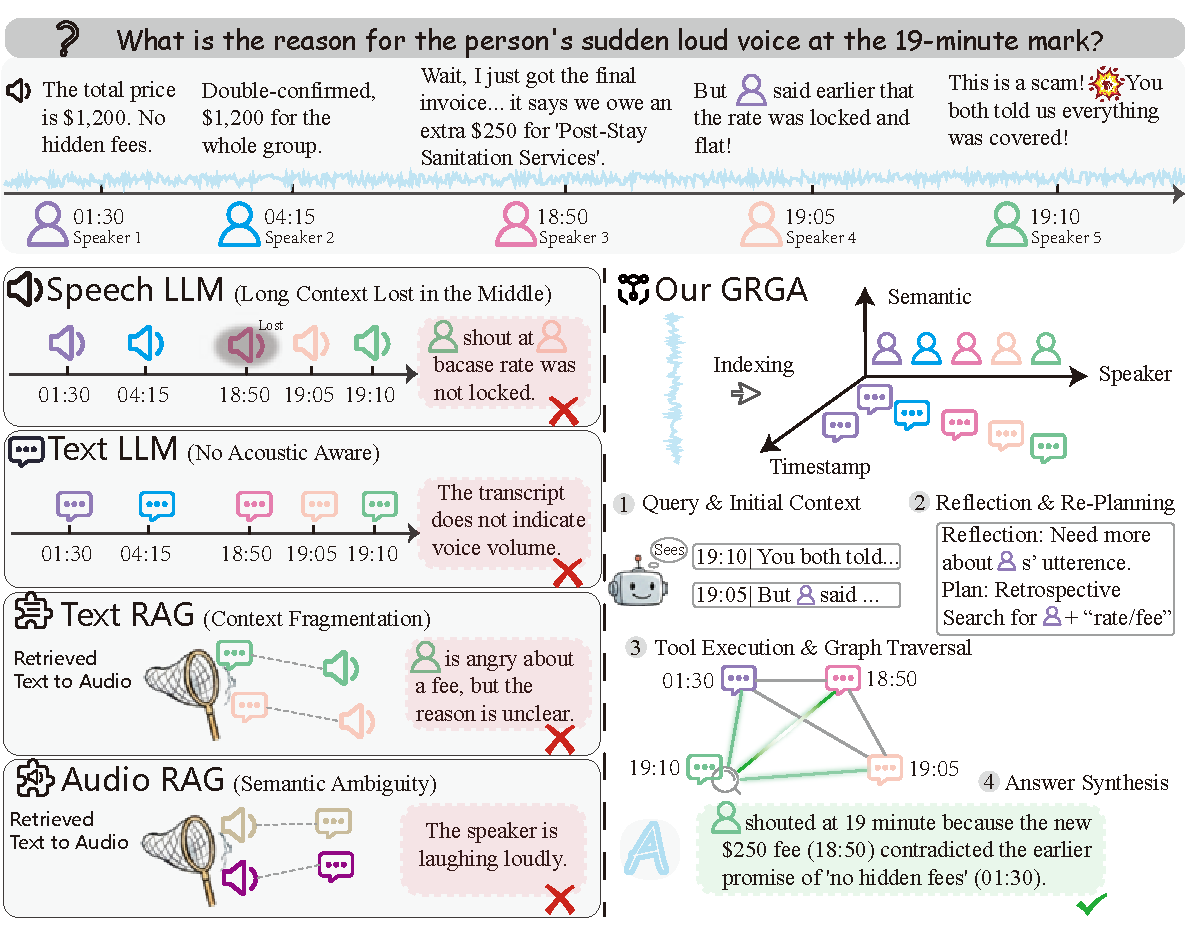
\includegraphics[width=\linewidth,height=4.86cm,keepaspectratio]{intro.pdf}\\[-0.12em]
      {\tiny\color{ACLDark}GRGA retrieves across semantic, speaker, and timestamp dimensions.}
    \end{column}
  \end{columns}
\end{frame}

%% ============================================================
%%  SLIDE 3 ─ LongAudioQA Dataset
%% ============================================================
\begin{frame}[t]{LongAudioQA: Benchmarking Long-form Audio Meeting QA}
  \vspace{-0.08cm}
  \begin{columns}[T]
    \begin{column}{0.40\textwidth}
      {\small\textbf{\color{ACLBlue}Three Sub-corpora}}\\[0.18em]
      \scriptsize
      \setlength{\tabcolsep}{4pt}
      \renewcommand{\arraystretch}{1.08}
      \begin{tabular}{lcr}
        \toprule
        \textbf{Dataset} & \textbf{Dur.} & \textbf{\#Q\&A}\\
        \midrule
        AliMeeting & 14.9\,h & 3,013\\
        AMI Meeting & 18.2\,h & 3,243\\
        DailyTalk & 21.6\,h & 10,200\\
        \bottomrule
      \end{tabular}
      \vspace{0.28cm}

      {\small\textbf{\color{ACLBlue}Five Question Types}}\\[0.18em]
      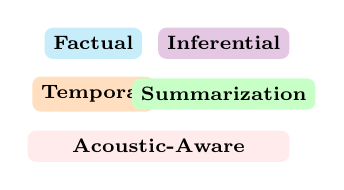
\begin{tikzpicture}[
        every node/.style={rounded corners=3pt,inner sep=3.2pt,font=\scriptsize\bfseries},
        xscale=0.92, yscale=0.86]
        \node[fill=cyan!22] at (0.9,2.0) {Factual};
        \node[fill=violet!22] at (2.7,2.0) {Inferential};
        \node[fill=orange!25] at (0.9,1.25) {Temporal};
        \node[fill=green!22] at (2.7,1.25) {Summarization};
        \node[fill=pink!32,text width=3.1cm,align=center] at (1.8,0.48)
          {Acoustic-Aware};
      \end{tikzpicture}

      \vspace{0.22cm}
      \begin{beamercolorbox}[wd=\linewidth,rounded=true,sep=0.12cm]{block body}
        {\scriptsize
        \textbf{Quality control:} hybrid LLM + human annotation;
        $\kappa{=}0.91$; timestamp IoU $>{0.9}$.}
      \end{beamercolorbox}
    \end{column}

    \begin{column}{0.58\textwidth}
      \centering
      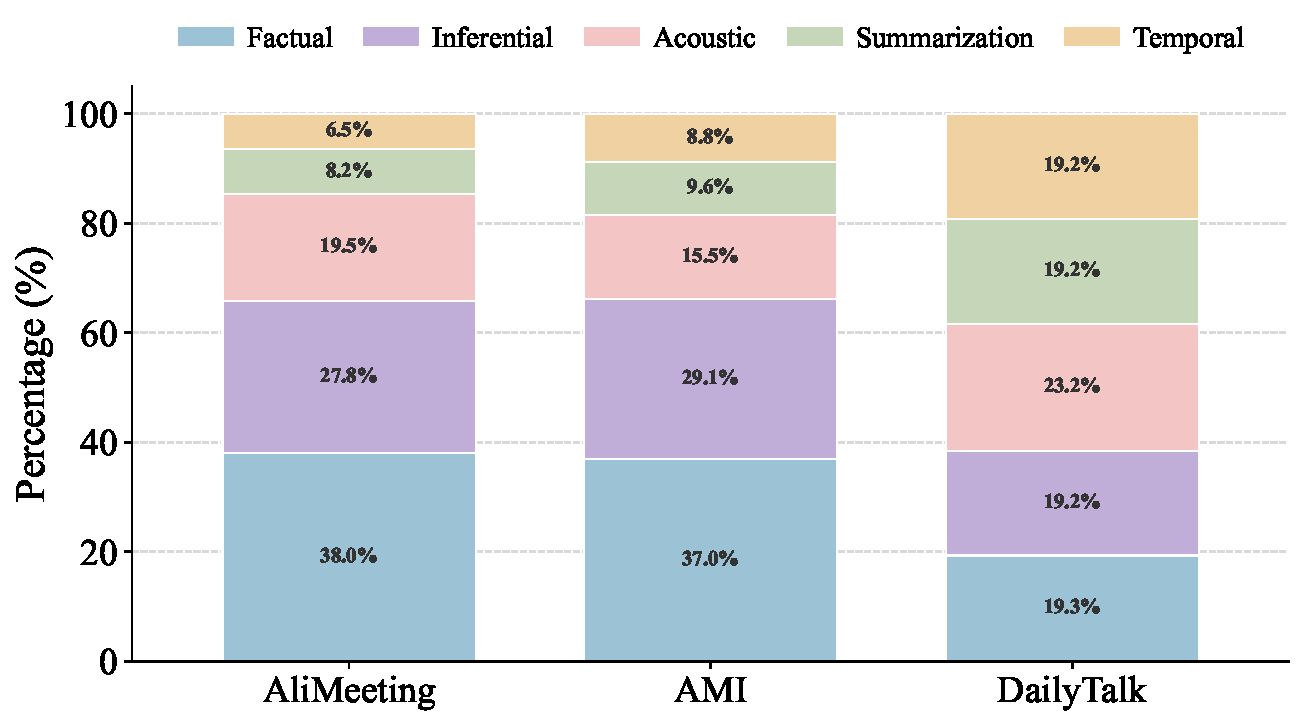
\includegraphics[width=0.82\linewidth,height=3.35cm,keepaspectratio]{qa_distribution.pdf}\\[-0.03em]
      {\footnotesize\color{ACLDark}
        Distribution across all three corpora.\\[0.20em]}
      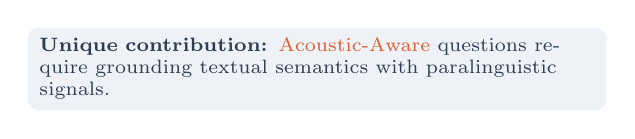
\begin{tikzpicture}
        \fill[ACLGray,rounded corners=4pt]
          (0,0) rectangle (7.35cm,1.05cm);
        \node[align=left,text width=7.05cm,font=\scriptsize,ACLDark]
          at (3.675cm,0.525cm){%
          \textbf{Unique contribution:}
          \textcolor{ACLOrange}{Acoustic-Aware} questions require grounding
          textual semantics with paralinguistic signals.};
      \end{tikzpicture}
    \end{column}
  \end{columns}
\end{frame}

%% ============================================================
%%  SLIDE 4 ─ GRGA Architecture
%% ============================================================
\begin{frame}[t]{GRGA Architecture: Multi-dimensional Graph + POMDP Planning}
  \vspace{-0.06cm}
  \begin{columns}[T]
    \begin{column}{0.62\textwidth}
      \centering
      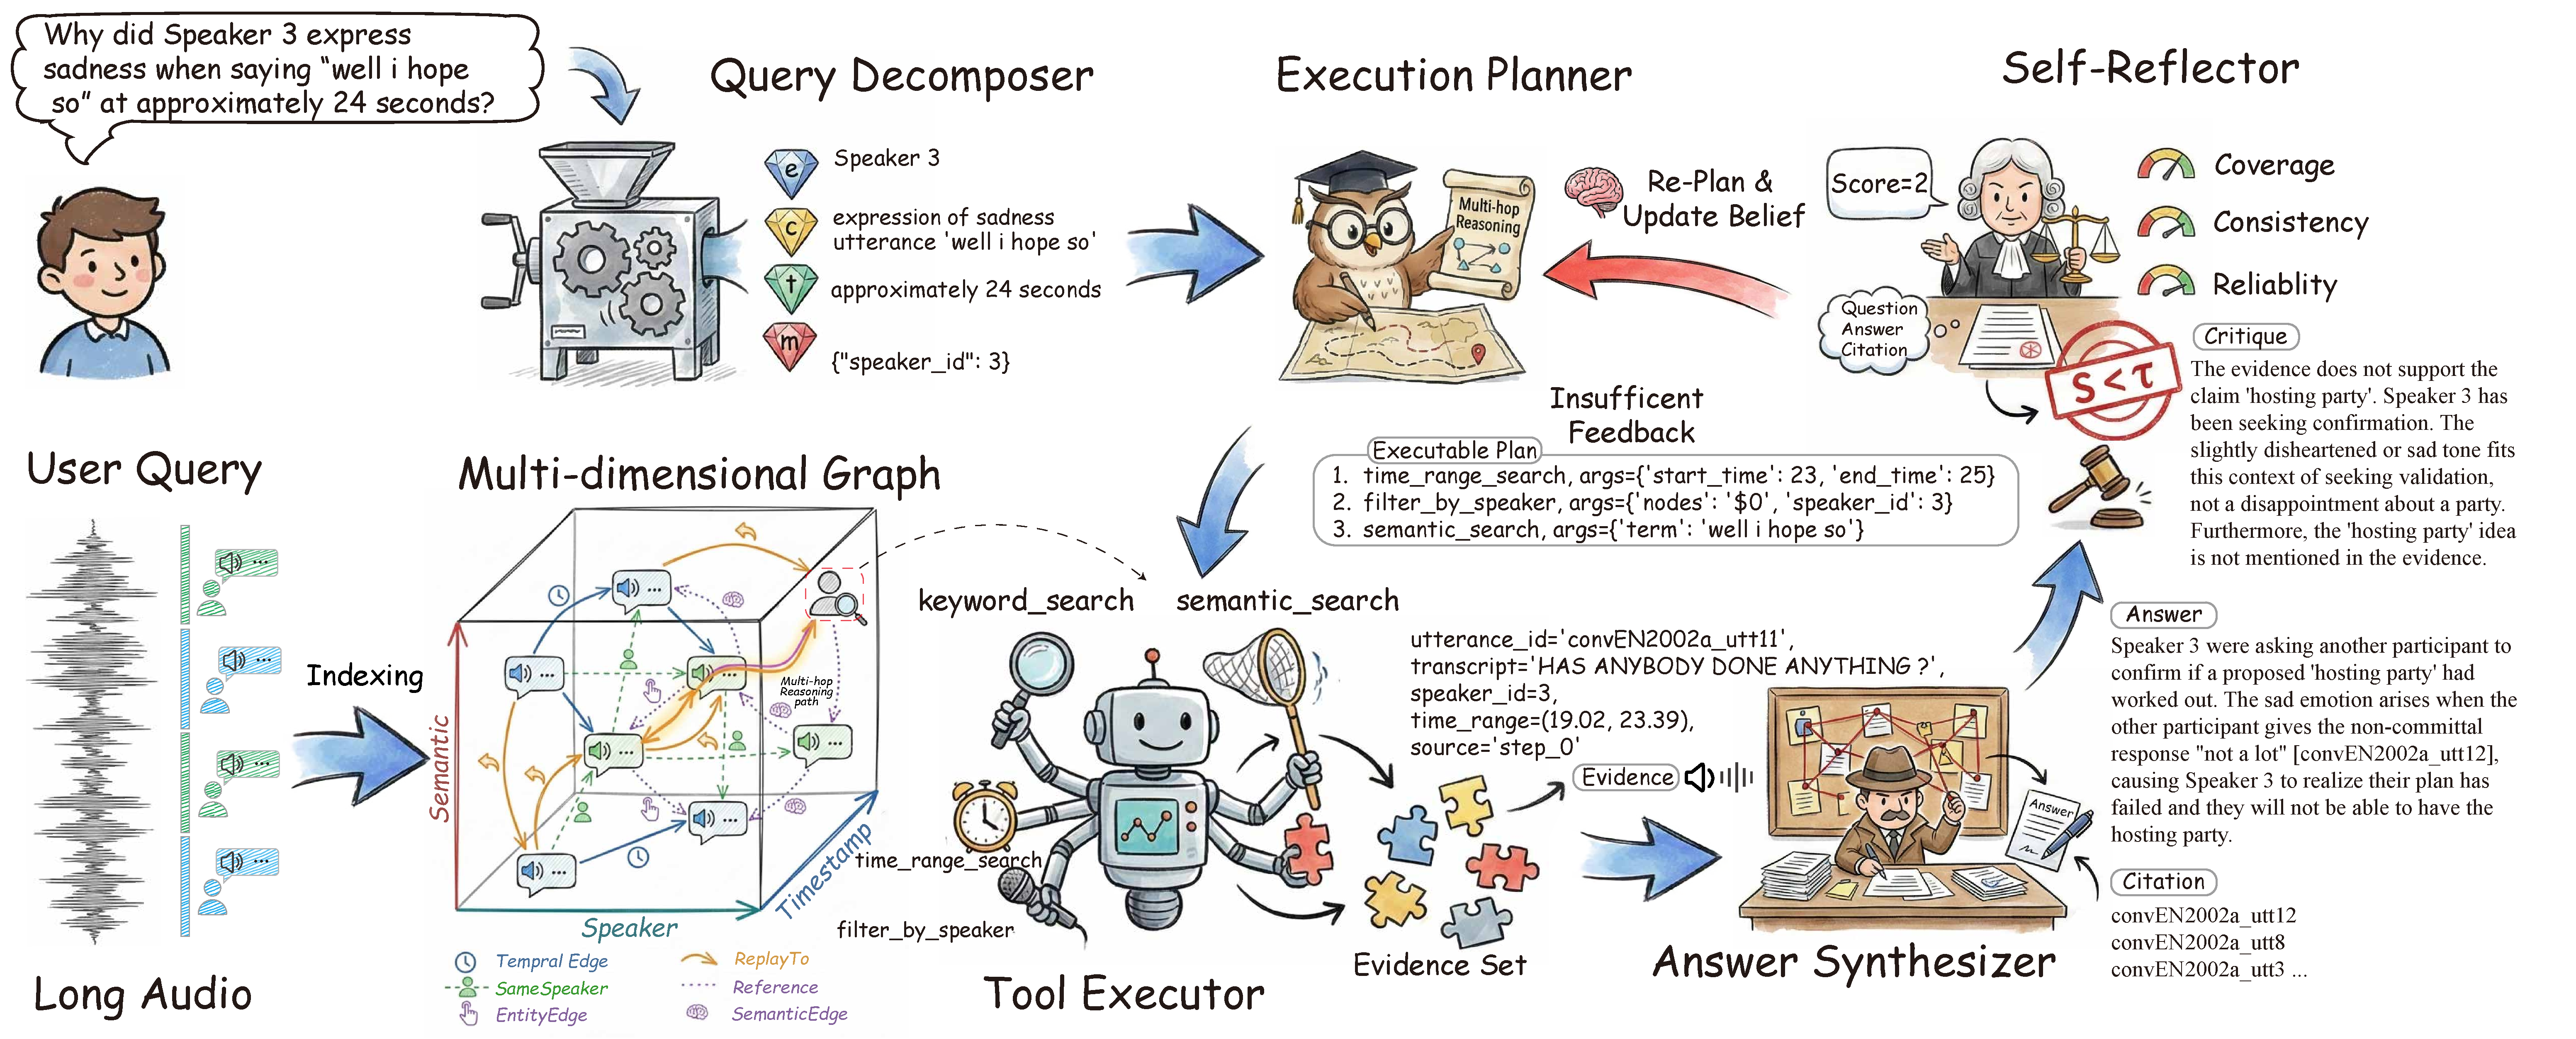
\includegraphics[width=\linewidth,height=6.0cm,keepaspectratio]{method.pdf}
    \end{column}

    \begin{column}{0.36\textwidth}
      \textbf{\color{ACLBlue}Meeting Graph $\mathcal{G}$}\\[-0.05em]
      \footnotesize
      \textbf{Nodes} $v_i$: utterances with text, speaker, timestamp, and audio.\\[0.22em]
      \textbf{Edge types:}
      \begin{itemize}\tightitems
        \item $e_{\text{temp}}$: adjacent turns
        \item $e_{\text{reply}}$: replies within $\Delta t<5$s
        \item $e_{\text{spk}}$: same-speaker links
        \item $e_{\text{ent}}$: shared keywords
        \item $e_{\text{sem}}$: LLM coreference chains
      \end{itemize}
      \vspace{0.25em}
      \textbf{\color{ACLBlue}Agent as POMDP}\\[-0.05em]
      {\scriptsize
      $\mathcal{M}=\langle\mathcal{S},\mathcal{A},\mathcal{T},\mathcal{R},\Omega,\mathcal{O},\gamma\rangle$}
      \begin{itemize}\tightitems
        \item Belief $b_t$: query + history
        \item Policy $\pi$: ICL-guided LLM
        \item Reward: Self-Reflector score
      \end{itemize}
      \vspace{0.12em}
      {\scriptsize\color{ACLDark}
        Pipeline: VAD $\to$ ASR $\to$ diarization $\to$ profile LLM.}
    \end{column}
  \end{columns}
\end{frame}

%% ============================================================
%%  SLIDE 5 ─ GRGA Planning Process
%% ============================================================
\begin{frame}[t]{GRGA Planning: A Cognitive ``Search-Reason-Verify'' Loop}
  \vspace{-0.04cm}
  \centering
  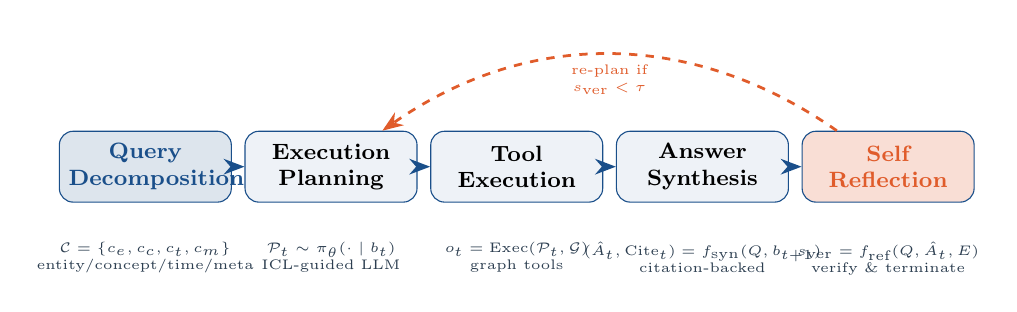
\begin{tikzpicture}[
    node distance=0.06cm and 0.16cm,
    box/.style={rounded corners=5pt,draw=ACLBlue,fill=ACLGray,
                text width=1.95cm,align=center,minimum height=0.9cm,
                font=\footnotesize\bfseries},
    arrow/.style={-Stealth,ACLBlue,line width=1pt},
    label/.style={font=\tiny,ACLDark,align=center}]

    \node[box,fill=ACLBlue!15] (dec)
      {\color{ACLBlue}Query\\Decomposition};
    \node[box,right=of dec] (plan)
      {Execution\\Planning};
    \node[box,right=of plan] (exec)
      {Tool\\Execution};
    \node[box,right=of exec] (syn)
      {Answer\\Synthesis};
    \node[box,fill=ACLOrange!20,right=of syn] (ref)
      {\color{ACLOrange}Self\\Reflection};

    \draw[arrow] (dec) -- (plan);
    \draw[arrow] (plan) -- (exec);
    \draw[arrow] (exec) -- (syn);
    \draw[arrow] (syn) -- (ref);
    \draw[arrow,dashed,ACLOrange] (ref) to[bend right=35]
      node[below,label,ACLOrange]{re-plan if\\$s_\text{ver}<\tau$} (plan);

    \node[label,below=0.38cm of dec]
      {$\mathcal{C}=\{c_e,c_c,c_t,c_m\}$\\entity/concept/time/meta};
    \node[label,below=0.38cm of plan]
      {$\mathcal{P}_t\sim\pi_\theta(\cdot\mid b_t)$\\ICL-guided LLM};
    \node[label,below=0.38cm of exec]
      {$o_t=\text{Exec}(\mathcal{P}_t,\mathcal{G})$\\graph tools};
    \node[label,below=0.38cm of syn]
      {$(\hat{A}_t,\text{Cite}_t)=f_\text{syn}(Q,b_{t+1})$\\citation-backed};
    \node[label,below=0.38cm of ref]
      {$s_\text{ver}=f_\text{ref}(Q,\hat{A}_t,E)$\\verify \& terminate};
  \end{tikzpicture}

  \vspace{0.14cm}
  \begin{columns}[T]
    \begin{column}{0.48\textwidth}
      \textbf{\color{ACLBlue}Action Space (4 Graph Tools):}
      \footnotesize
      \begin{itemize}\tightitems
        \item \textbf{Semantic Search}: retrieve node text
        \item \textbf{Temporal Filter}: constrain time ranges
        \item \textbf{Graph Traversal}: follow speaker/semantic links
        \item \textbf{Audio Access}: inspect acoustic cues
      \end{itemize}
    \end{column}
    \begin{column}{0.50\textwidth}
      \textbf{\color{ACLBlue}Key Design Choices:}
      \footnotesize
      \begin{itemize}\tightitems
        \item \textbf{Training-free}: LLM policy via in-context learning
        \item \textbf{Adaptive depth}: shallow for factual, deeper for temporal/inferential
        \item \textbf{Self-correction}: reflection filters low-evidence answers
      \end{itemize}
    \end{column}
  \end{columns}
\end{frame}

%% ============================================================
%%  SLIDE 6 ─ Main Results
%% ============================================================
\begin{frame}[t]{Experimental Results: GRGA Outperforms All Baselines}
  \vspace{-0.06cm}
  {\scriptsize
  \setlength{\tabcolsep}{3.15pt}
  \renewcommand{\arraystretch}{1.08}
  \resizebox{\linewidth}{!}{%
  \begin{tabular}{l l ccccc ccccc}
    \toprule
    \multirow{2}{*}{\textbf{Category}} &
    \multirow{2}{*}{\textbf{Method}} &
    \multicolumn{5}{c}{\textbf{AliMeeting}} &
    \multicolumn{5}{c}{\textbf{AMI Meeting}} \\
    \cmidrule(lr){3-7}\cmidrule(lr){8-12}
    & & \textbf{Fact.} & \textbf{Infer.} & \textbf{Temp.} & \textbf{Summ.} & \textbf{Acou.}
      & \textbf{Fact.} & \textbf{Infer.} & \textbf{Temp.} & \textbf{Summ.} & \textbf{Acou.} \\
    \midrule
    \multirow{2}{*}{\scriptsize Speech LLM}
      & Qwen3-Omni    & 47.7 & 63.5 & 38.3 & 32.7 & 11.7
                      & 53.6 & 46.7 & 37.3 & 43.6 & 14.1 \\
      & MiMo-Audio    & 48.0 & 64.6 & 38.3 & 29.4 & 15.7
                      & 53.6 & 44.1 & 37.1 & 41.5 & 17.9 \\
    \midrule
    \multirow{2}{*}{\scriptsize RAG}
      & BGE-M3 (text) & 43.2 & 29.7 & 31.6 & 15.4 & 18.5
                      & 32.6 & 24.6 & 23.8 & 25.4 & 25.3 \\
      & CLASP (audio) & 25.4 & 19.5 & 18.9 & 14.8 & 16.3
                      & 24.1 & 20.3 & 22.8 & 11.6 & 14.8 \\
    \midrule
    \rowcolor{rowgray}
    \textbf{Ours} & \textbf{GRGA}
      & \textbf{57.3} & \textbf{66.5} & \textbf{39.5} & \textbf{44.3} & \textbf{39.9}
      & \textbf{59.5} & \textbf{65.3} & \textbf{38.6} & \textbf{48.5} & \textbf{35.7} \\
    \bottomrule
  \end{tabular}}}

  \vspace{0.18cm}
  \begin{columns}[T]
    \begin{column}{0.48\textwidth}
      \footnotesize
      \textcolor{ACLBlue}{\textbf{Key Findings:}}
      \begin{itemize}\tightitems
        \item \highlight{+10\%} average gain over the best speech LLM on AMI.
        \item Inferential QA: \textbf{65.3\%} vs.\ Text RAG \textbf{24.6\%}.
        \item Acoustic QA: \textbf{39.9\%} vs.\ next-best \textbf{18.5\%}.
      \end{itemize}
    \end{column}
    \begin{column}{0.50\textwidth}
      \footnotesize
      \textcolor{ACLBlue}{\textbf{Why GRGA Wins:}}
      \begin{itemize}\tightitems
        \item Graph structure preserves multi-hop meeting dependencies.
        \item Audio access supports acoustic-aware evidence.
        \item Reflection suppresses low-evidence answers.
      \end{itemize}
    \end{column}
  \end{columns}
\end{frame}

%% ============================================================
%%  SLIDE 7 ─ Analysis
%% ============================================================
\begin{frame}[t]{Analysis: Human Evaluation \& Ablation Study}
  \vspace{-0.05cm}
  \begin{columns}[T]
    \begin{column}{0.46\textwidth}
      \textbf{\color{ACLBlue}Human Evaluation}\\[0.12em]
      \centering
      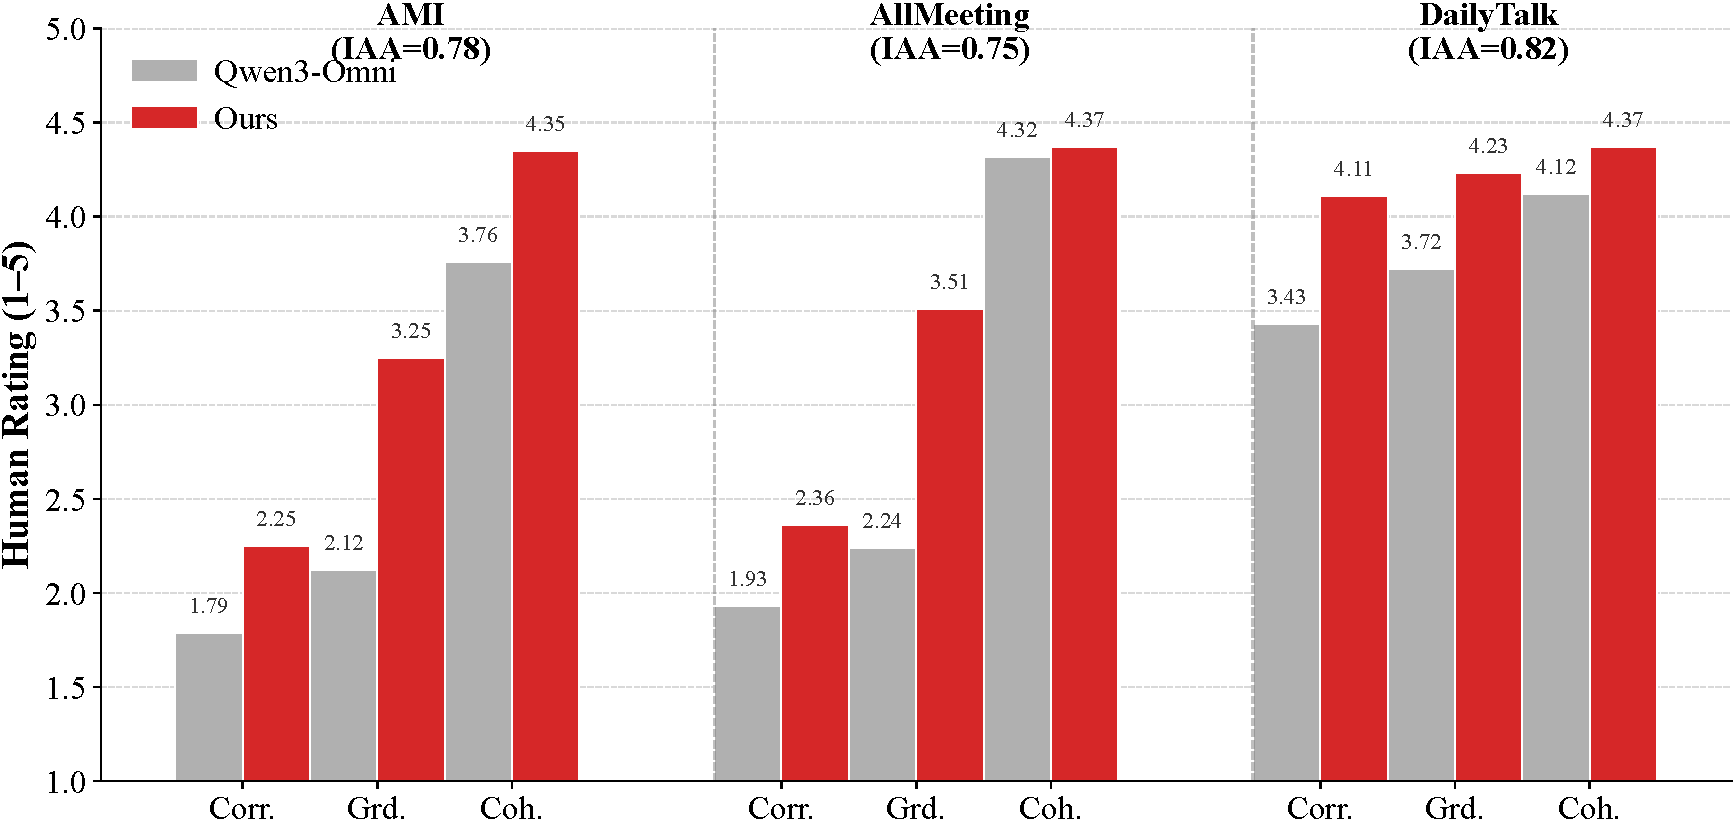
\includegraphics[width=0.90\linewidth,height=3.95cm,keepaspectratio]{human_eval.pdf}\\[0.15em]
      {\scriptsize\color{ACLDark}
        Blind evaluation on 150 queries (3 annotators, IAA$=0.78$).\\
        \alert{+0.97 Groundedness} confirms fewer hallucinations.}
    \end{column}

    \begin{column}{0.52\textwidth}
      \textbf{\color{ACLBlue}Ablation Study (AMI)}\\[0.12em]
      {\footnotesize
      \setlength{\tabcolsep}{3pt}
      \renewcommand{\arraystretch}{1.04}
      \begin{tabular}{lcc}
        \toprule
        \textbf{Setting} & \textbf{Avg.\,\%} & \textbf{$\Delta$}\\
        \midrule
        \textbf{Full GRGA} & \textbf{49.49} & --\\
        \midrule
        w/o Query Planner   & 44.68 & \textcolor{red}{$-4.80$}\\
        w/o Reflection      & 39.64 & \textcolor{red}{$-9.84$}\\
        w/o Graph Traversal & 38.21 & \textcolor{red}{$-11.27$}\\
        w/o Audio Access    & 34.71 & \textcolor{red}{$-14.78$}\\
        w/o Semantic Search & 16.28 & \textcolor{red}{$-33.21$}\\
        \bottomrule
      \end{tabular}}

      \vspace{0.22cm}
      {\footnotesize
      \textbf{\color{ACLBlue}Evidence Precision/Recall (AMI, $\pm2$s)}}\\[0.12em]
      {\footnotesize
      \begin{tabular}{lcc}
        \toprule
        \textbf{Method} & \textbf{P} & \textbf{R}\\
        \midrule
        Qwen3-Omni        & 25.7 & 27.3\\
        + Text RAG        & 56.9 & 65.2\\
        \textbf{+ GRGA}   & \textbf{76.2} & \textbf{69.7}\\
        \bottomrule
      \end{tabular}}
    \end{column}
  \end{columns}
\end{frame}

%% ============================================================
%%  SLIDE 8 ─ Conclusion
%% ============================================================
\begin{frame}[t]{Conclusion}
  \vspace{-0.06cm}
  \begin{columns}[T]
    \begin{column}{0.58\textwidth}
      \begin{block}{\textcolor{white}{Contributions}}
        \footnotesize
        \begin{enumerate}\tightitems
          \item \textbf{LongAudioQA}: first large-scale long-form audio meeting QA
                benchmark with 16,456 Q\&A pairs across three corpora.
          \item \textbf{GRGA}: training-free agent that models heterogeneous audio
                as a multi-dimensional graph and plans iteratively.
          \item \textbf{Evaluation}: automatic + human studies show consistent
                gains over Speech LLM and RAG baselines.
        \end{enumerate}
      \end{block}

      \vspace{0.16cm}
      \begin{alertblock}{\textcolor{white}{Limitations \& Future Work}}
        \footnotesize
        \begin{itemize}\tightitems
          \item Noisy ASR/diarization can still corrupt graph evidence.
          \item Iterative planning is slower than single-turn RAG.
          \item Future: streaming QA and broader long-form audio domains.
        \end{itemize}
      \end{alertblock}
    \end{column}

    \begin{column}{0.40\textwidth}
      \vspace{0.04cm}
      \centering
      % Summary diagram
      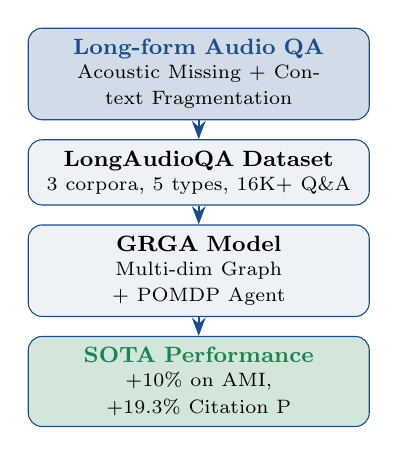
\begin{tikzpicture}[
        box/.style={rounded corners=5pt,draw=ACLBlue,fill=ACLGray,
                    text width=4.05cm,align=center,
                    font=\footnotesize,inner sep=4pt},
        arrow/.style={-Stealth,ACLBlue,line width=0.8pt}]
        \node[box,fill=ACLBlue!20] (prob)
          {\textbf{\color{ACLBlue}Long-form Audio QA}\\[-0.1em]
           {\scriptsize Acoustic Missing + Context Fragmentation}};
        \node[box,below=0.24cm of prob] (data)
          {\textbf{LongAudioQA Dataset}\\[-0.1em]
           {\scriptsize 3 corpora, 5 types, 16K+ Q\&A}};
        \node[box,below=0.24cm of data] (model)
          {\textbf{GRGA Model}\\[-0.1em]
           {\scriptsize Multi-dim Graph + POMDP Agent}};
        \node[box,fill=ACLGreen!20,below=0.24cm of model] (res)
          {\textbf{\color{ACLGreen}SOTA Performance}\\[-0.1em]
           {\scriptsize +10\% on AMI, +19.3\% Citation P}};
        \draw[arrow] (prob)--(data);
        \draw[arrow] (data)--(model);
        \draw[arrow] (model)--(res);
      \end{tikzpicture}

      \vspace{0.25cm}
      {\footnotesize\color{ACLDark}
        \textbf{Code \& Data:}\\
        \url{github.com/tangquanwei/GRGA}}
    \end{column}
  \end{columns}
\end{frame}

\end{document}
